\chapter{バリデーション}
\section{実験概要}
制作された修士作品が実際にはどのように体験されるのかについてインタビューを実施し、作品として何が達成されたのかについて考察する。

\section{目的}

\section{実施方法}
\subsection{Video Cued-Recall メソッド}
インタラクティブ作品の評価方法にはさまざまな評価が存在するが、本作品を評価する上では、体験時、体験者がどのようなことに注意を向け、どのような行動を取ったかについて精緻に振り返る必要がある。そのため本研究では、体験者に体験時のようすをできるだけ詳細に表現してもらうため、Video Cued-Recallというメソッドを用いてデータの収集を行なった。 Video Cued-Recallとは、体験時のようすが記録された映像を視聴しながら、体験者本人が映像を手がかりに作品での体験を回顧し、言語化する方法である\cite{Costello2005}。インタビューを通して回顧するよりも詳細に体験を振り返ることができ、また体験しているそのときに体験のようすについて語ってもらう方法よりも、自然な体験について記述できることがその利点として挙げられる。

\subsection{参加者について}
インタビューは、FabCafe Nagoyaでの展示に際して、4名の体験者を対象に実施した。ただし、うち1名は「Relation」の体験時、トラッキングの精度が著しく低下していたため、1つ目に体験した「Familiar / Strange」の体験についてのみ調査の対象とした。

\subsection{データ収集}
参加者にはまず、調査の大まかな流れについて説明し、撮影についての許諾を得た。コンセプトの説明が自然な体験に影響することを避けるため、作品の体験の前にはコンセプトや具体的な作品の内容については説明せず、トラッキングされた手が次々に形を変えていくこと、手の形が表示された状態から始まり、再びもとの手の形に戻るループ構造のある作品であること、というインタビューに必要な最低限の構造のみ伝えた。

体験のようすは、手もとのハンドトラッキングを行うカメラ映像、現在時刻、体験者が実際に見ているスクリーンの映像が図\ref{fig:record_monitor}のようにレイアウトされて記録される。

\begin{figure}[H]
  \centering
  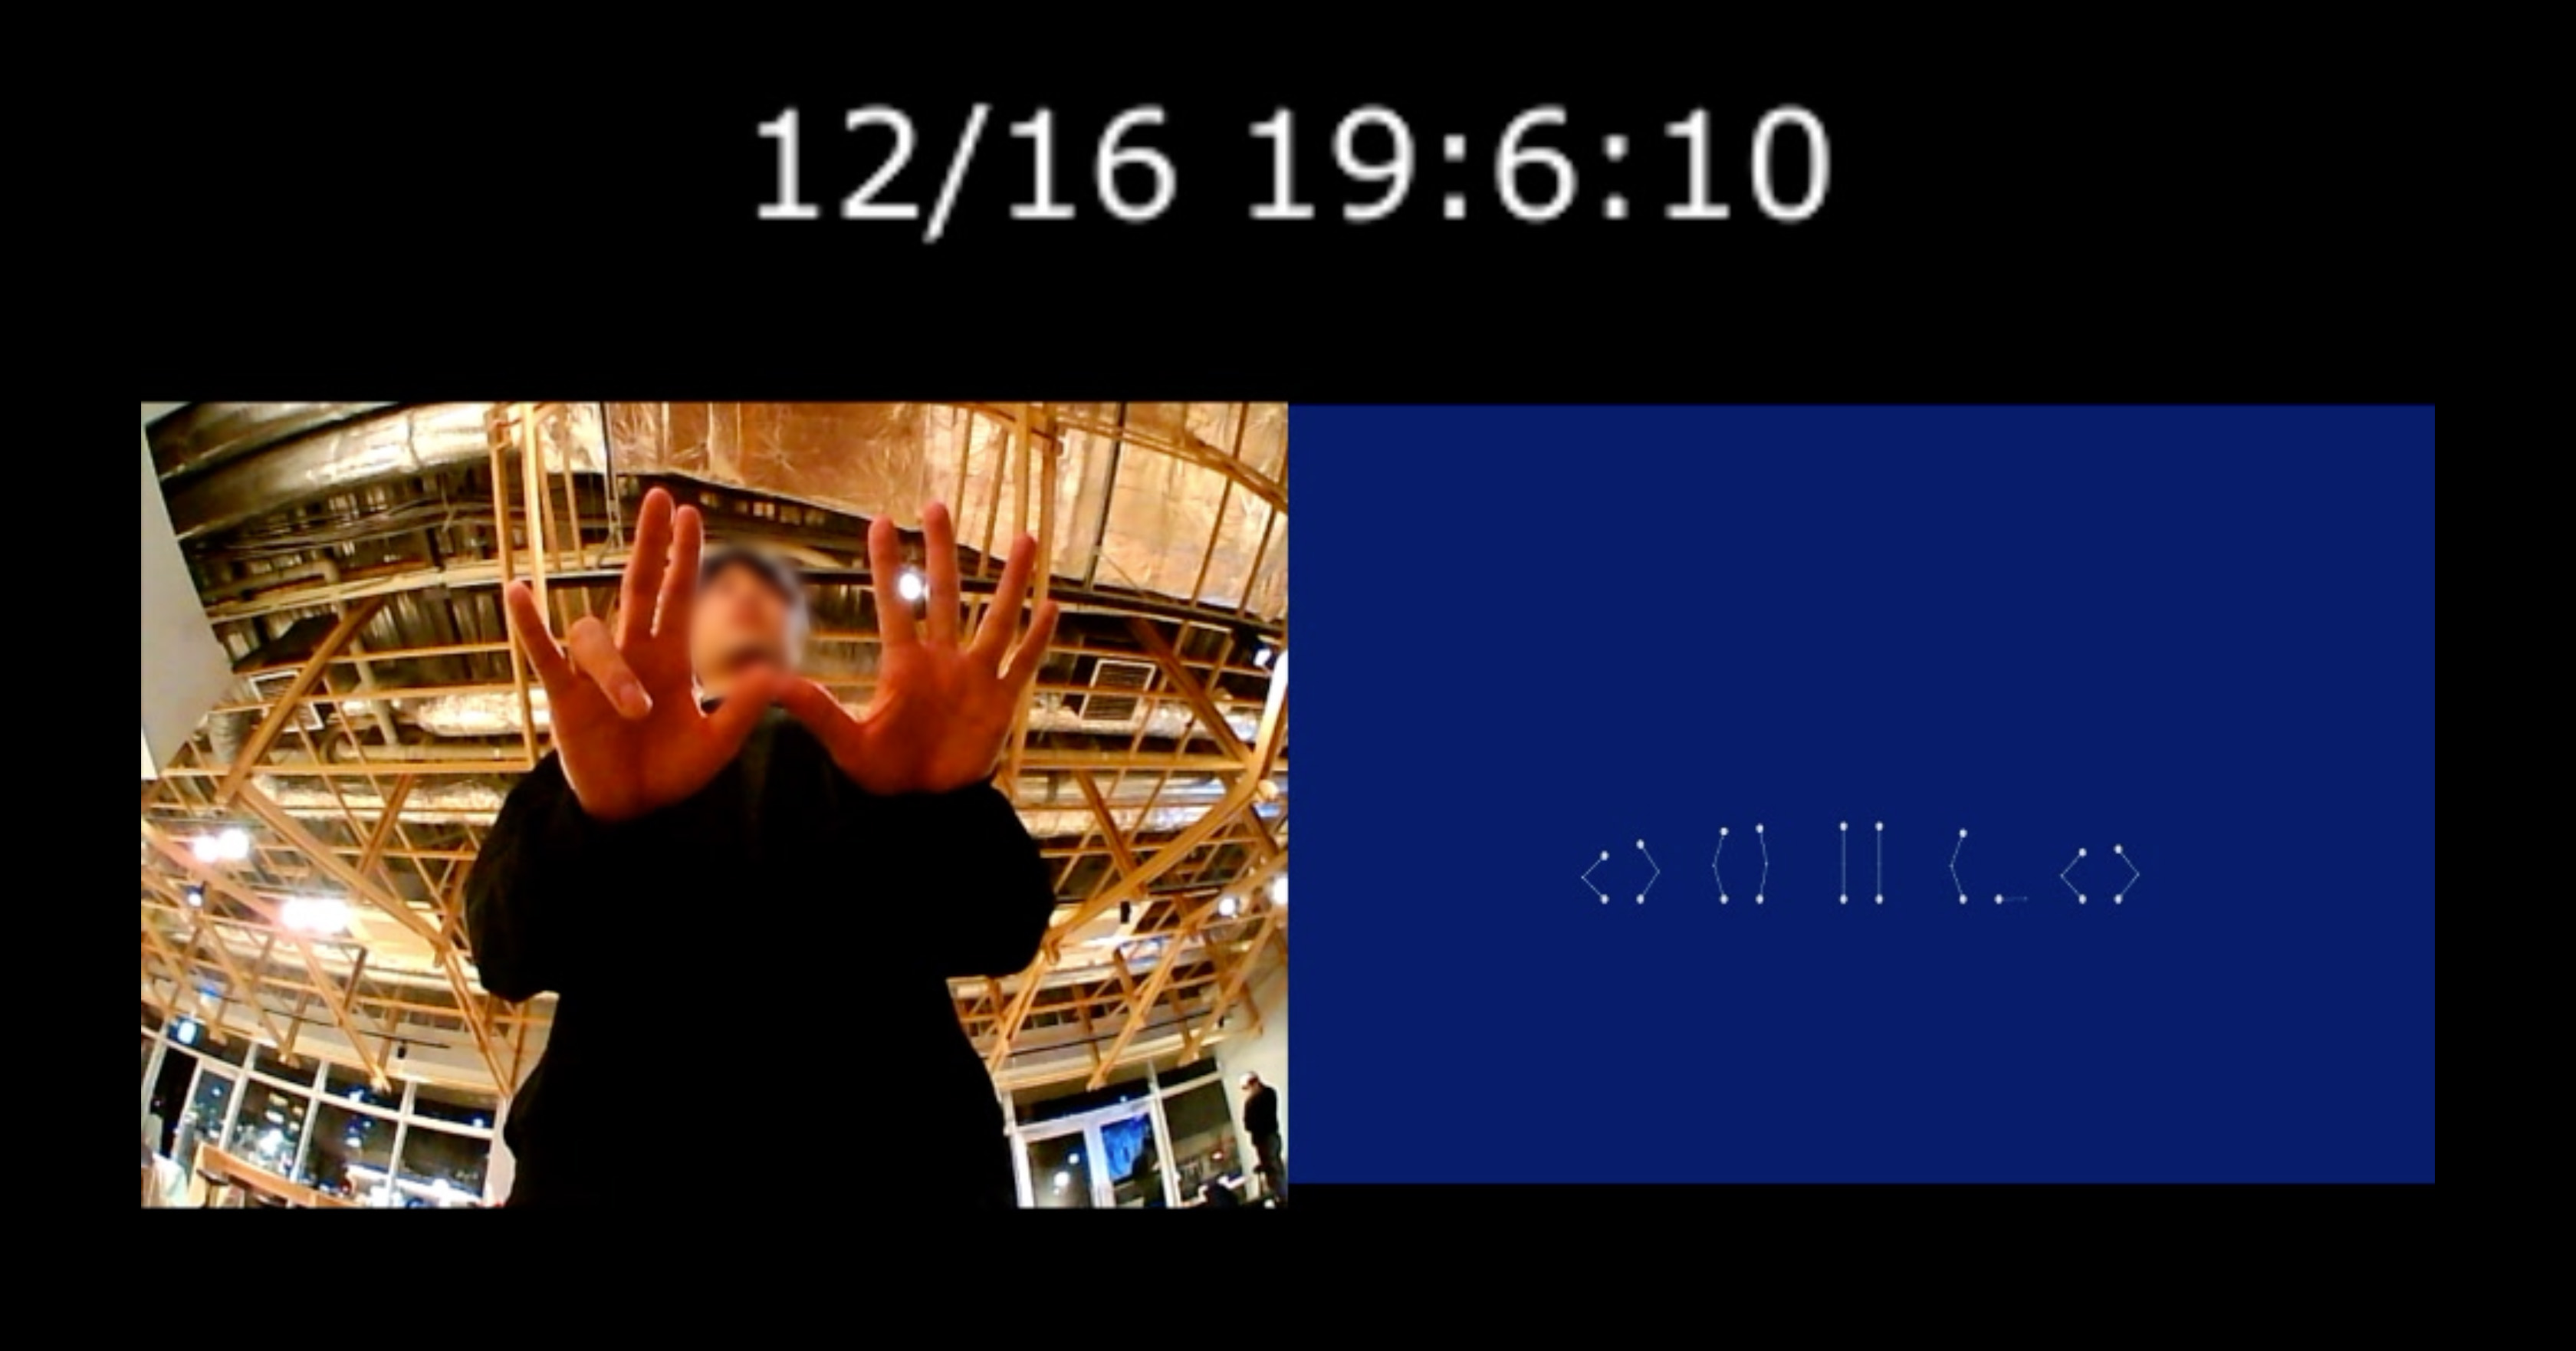
\includegraphics[width=15cm]{img/record_monitor.jpg}
  \caption{体験のようすの記録映像}
  \label{fig:record_monitor}
\end{figure}

作品体験が終了した後、体験者自身が上記の記録映像を視聴しながら、作品体験時のようすを詳細に言語化する振り返り作業を依頼する。この時点では、そのとき考えていたことや、試行した事柄とその理由など、作品体験を終えた今思う感想ではなく、その当時経験していたことについて言語化してもらうよう促した。体験者は、自由に映像を停止したり、巻き戻すことができる。
作業の際は研究実施者も同席しているが、調査を実施する上でのトラブルが生じない限り、原則体験者個人で振り返る。\\
その後、前の振り返りの作業や体験のようすを踏まえて、研究実施者が半構造化インタビューを実施することで、より精緻に作品体験のようすを振り返るとともに、体験を終えた上での感想などについて伺った。
いずれもループ構造の作品であるため、1周するまでの期間をその調査対象とした。ただし、作品「Relation」については、一周するための達成条件がシビアであることから、体験の終了は3分以上体験することを目安に、いつでも体験を終了してよいこととした。

\subsection{データの記録}
インタビューから言語化された体験時の回想を、図\ref{fig:spreadsheet}のようにスプレッドシート上に時系列で記録した。シート上には、1秒ごとのタイムスタンプ(日本標準時)、その時刻でのトラッキングの状況(右手、左手、全体)、その時刻での出力内容を示すシーン情報、並びに発言内容が記録されている。また、その後に行ったインタビューについては文字起こしをしてテキストデータで記録した。
\begin{figure}[H]
  \centering
  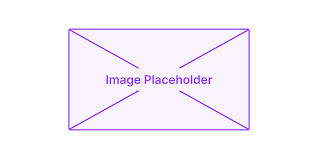
\includegraphics[width=15cm]{img/placeholder.png}
  \caption{発話情報が記録されたスプレッドシート}
  \label{fig:spreadsheet}
\end{figure}

\section{結果}
以下では、参加者の体験時の映像とそれをみながら体験者自身が行った回想、そして、インタビューを通して得られた意見から、それぞれの参加者が「Familiar / Strange」、「Relation」をそれぞれどのように体験していたのかについて説明する。

\subsubsection{Familiar / Strange}
\subsubsection*{参加者1}
参加者1の手指の動きをみると、scene0からscene1にかけての、手が指ごとに離れていく過程を確かめる中では、手を握りしめたり、開いたりする動作が見られるが、scene1以降、関節が減り、左右の指で1セットのまとまりが明確になってくると、指を一本一本曲げる動きをするように変化した。手指の単位で分かれる「Scene1」から「Scene6」にかけては、どの指がどの指に対応しているのかについての「確認」を主に行なっていたと語る。
\begin{quote}
  どれがどの場所なんだろうって、最初は手の形になっているのでわかるんだけど、まぁそれがずれていってどれがどれかなっていうのを結構確認してたかな。
\end{quote}
しかしscene7になると、途端に握り拳を作る動きが多くなる。また、右手と左手を交互に握ったり、指一本単位でも、左右で同じ位置の指を曲げる動きが現れる。体験を振り返って、「干渉するイメージが強くなった」ことについて語る。
\begin{quote}
  今まで二つ単位で独立してたのが全部つながってバネみたいになって、お互いがお互いに干渉するイメージが強くなったかな。全部握ったら、全部閉じるんだ、みたいな。
\end{quote}
そして、「干渉」構造に気づいた後のscene7以降も手指の動きに注目すると、左右の指を同時に動かして「形を作る」ことに目的意識が生じていると考えられるような動きが、前半よりも増えたように見える。そして最後に両手を翻して、手を裏向きにした状態でもトラッキングができているかについて確認しているようすだった。\\
\subsubsection*{参加者2}
参加者2は最初、グー、チョキ、パーといった手全体でできる形を通して、「自分の手と、モニターに写っている手が、どれぐらい親和性高く動くのか」について確かめていた。また、しばらくは手を高くあげたり、下げたり、また両手を重ねたりすることで、トラッキングができる領域や認識精度の限界について確かめていた。Scene3から4にかけては、「親和性から離れていく感じ」があると語る。
\begin{quote}
  ここら辺からちょっと違和感というか、親和性を確かめてたのに、その親和性から離れてく感じがしてた。今の自分の手と、こっち側の手の連動が、してるんだけど離れている。自分の手じゃなくなる。
\end{quote}
また、参加者2は特に、手指を高速に動かすことで、どのスピードまで反応しうるかについても確かめていた。しかしScene7では、手指を高速に上下させても反応して動いている様子から体験中に「気持ちいい」と語っていた。
\begin{quote}
  ここら辺から自分が気持ちいい動きが探っていて。細かい動きを認識するなっていうのがここら辺でわかったから。ただ大きい動きになると、センサーの反応が悪くなったから、気持ちよく動く限りで、細かい微妙な動きをしたり。
\end{quote}
その後、再び元の手の形に戻るまでの過程では、腕全体を大きく振って指揮者のような動きをしながら、「俊敏な動きに対するトラッキングの時間差」を探っていたと語る。また、指揮者のような動きをしたことについては、「目視で手を見るだけでは認識することのできないような、指揮者の手の仕草など」が、「ビジュアルで出てくるとわかりやすい」といったことを想像していたと語った。

\subsubsection*{参加者3}
参加者3は最初、フレーミングする手のジェスチャーをするなどして、形を作っていた。しばらくして、自分の動きとは関係なくシーンが遷移していることに気づくと、手を動かすことを止めて「自分が動かなくても動く」ということを確かめていた。ほかにも、「徐々に、点がなくなっていくのを見ながら楽し」むなど、手指を動かさなかったときのシーン遷移についての感想が多かった。しかしその一方で、他の参加者1、2とは異なり、指を一本一本動かし、どこがどの指であるかを確かめるような動きは少なかった。
scene3から4に遷移する過程で「こうやってしたら(両手を開いて親指と人差し指をつなげ、三角形を作る)くっつくのかな、みたいなことをやっていました。特にくっつかなかった。」「(指を交差させて)こうやってやったら変わるのかな」と、「形を作る」ことができるのかについて試行していたが、結果「作れなかった」と認識してからは、手を開いた状態で、カメラに手を近づけたり遠ざけたり、手首を回すような動きをとっていた。そして、体験については「途中で飽きていた」と振り返った。インタビューにおいてその理由を尋ねると、「反応が変わらない」ことがその理由であると語った。
\begin{quote}
  関節五個あった時は楽しかったんですよ。それが一個になって、あれ、なんか手を動かしても広げなくても変わらない、やってもやらなくても反応が変わらない。ならやらない、みたいな。  
\end{quote}

\subsubsection{Relation}
\subsubsection*{参加者1}
参加者1は最初、マトの存在には気づかず、「左にボールがあったら右の方に移動させようとか、右にあったら左に移動させてみようとか」と、左右にボールを移動させることについて目的意識を持って、球を操ろうと試みていた。しばらくすると、ボールが偶然球にあたり、それからマトに当てることを目指すようになった。これについては、「ちゃんと当てようと思ってたんだけど、なかなか当たら」なかったと振り返る。\\
手指の動きに注目すると、マトに当てることを目指すようになってからは手指の動かし方には大きな変化が見られなかった。途中、マトの方に向けて手をはらうような動きをしてみたり(17:31:05)、手のひらを裏返した状態で動かそうと試みる(17:31:08)が、思うような挙動はしなかったためか、手指の姿勢は元の姿勢へと戻った。
\subsubsection*{参加者2}
参加者2は、途中までマトの存在に気づかないまま体験していた。その中で、ボールの投げ上げに「どれぐらいの動きでどれぐらいバウンドするのか」、「ボールをちょっと滞在させたい」「ちょっとなだらかな面を作ろう」とする、波打つような動きを作るなど、マトに当てるということ以外での目的設定をしながら身体を動かしていた。途中、
\begin{quote}
  ちょっとコツを掴もうと思って、一回動きを静かにして、動きのコツを探してたけど、なかなか難しくて。左に投げたいのに、左にあまり流れない、みたいな。角度傾斜をつけて、ある程度投げたい位置まで来たら、上にあげたらいいんじゃないかなっていう。無理くり、投げる角度でコントロールするのは難しいな、と。  
\end{quote}
と、投げ上げに関して「コツを掴もう」としたことについても振り返っている。しかし一方で、ボールを投げ上げてマトに当てるということに目的意識が芽生えてからは、波打つような動きを作るときとは違って「イライラ」していた感覚について語っている。その理由として「反応の鈍さ」に言及する。
\begin{quote}
  投げるときの反応が鈍くて、ちょっとイライラしてた。前の手のトラッキングだけとは違って、線が入ることで、もどかしいっていうか。  
\end{quote}
\subsubsection*{参加者3}
参加者3はボールの出現に際して「トランポリンみたい」(13:06:14)だという見立てから、高く飛ばしてみるということを試みていた。その後、ボールが画面の端から転がり落ちた(13:06:22)ことを確認して、「落ちるのは良くなさそう」と捉え、「次からは落とさないようにしよう」と制約をかけるようになった。さらに、高く飛ばしたボールが偶然マトに当たることを繰り返す(13:06:19 / 13:06:21 / 13:06:36)中で、「そうかあれは当てればいいのか」と認識し、マトに当てることを目的として設定するようになった。手指の対応関係については、端から小指、中心に両手の親指となる順で並べられているという構造については認識していたと振り返る一方で、体験の途中では手のひらを上に向け、掬い上げるような動きをしてボールを投げ上げる動きを試みていた。
しかし、しばらく当たらない状態が続き、諦めて体験が終了した。